El control de accesos físico, el cual puede ser un torniquete o una chapa eléctrica montada en alguna puerta, se diseñó utilizando una tarjeta raspberry pi, dicha tecnología se le montó un sistema Elixir Nerves junto con un frameworks Phoenix Liveview, ambos el elixir Nerves como el Phoenix Liveview son aglutinados utilizando la técnica ``PONCHO''. Además se utilizarón dos técnicas de captura de eventos de los lectores:

\begin{itemize}
\item Lectura por evento.- Para lo cual se utiliza una libreria que captura los eventos del sistema operativo que llegan al puerto \textbf{/dev /inputX} del dispositivo.
\item Lectura por HID.- Se utiliza la propiedad de HID de los dispositivos capturando a través de un streaming las lecturas del dispositivo, en este caso a través de los puertos \textbf{/dev /hidX} del sistema operativo.
\end{itemize}

Empezaremos con describiendo de manera genérica como trabaja un proyecto poncho que glutinará los otros dos subproyectos.

\section{Proyecto Elixir Poncho con firmware elixir nerves y UI de Phoenix Liveview}

Un proyecto poncho es una estructura para la elaboración de proyectos grandes, en donde conceptualmente se dividen las funciones, en este caso en dos partes principales como se muestra en la figura \ref{cap2:001}.


\begin{figure}[htb]
\centering
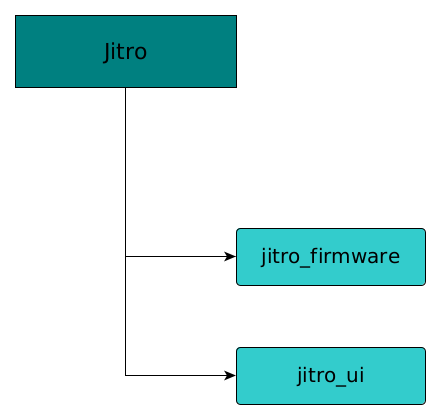
\includegraphics[width=0.4\textwidth]{capitulo2/jitro.png}
\caption{Estructura General del Proyecto JITRO de SMARTEST}
\label{cap2:001}
\end{figure}

\subsection{Estructura base del proyecto}

Primero crearemos el directorio en el cual se harán los dos subproyectos, tanto el de firmware como el de ui.

\begin{lstlisting}[language=bash]
$ mkdir Jitro 
$ cd Jitro
\end{lstlisting}

Ahora estableceremos el nombre del proyecto, en este caso será jitro\footnote{Por si tienen curiosidad jitro proviene del idioma construido Lojban y significa control}.

\begin{lstlisting}[language=bash]
$ export NOMBRE_PROYECTO=jitro
\end{lstlisting}

Crearemos tambien el archivo \textbf{README.md} con información para cuando se suba a github.

\begin{lstlisting}[language=bash]
$ echo "Proyecto creado por el departamento de I+D de SMARTEST \n Dr. Casimiro Gomez Gonzalez\\n 2021" > README.md
\end{lstlisting}


Posteriormente inicializamos el git

\begin{lstlisting}[language=bash]
$ git init && git add . && git commit -m "Inicial commit"
\end{lstlisting}

Ahora se crea el firmware 

\begin{lstlisting}[language=bash]
$ mix nerves.new "$NOMBRE_PROYECTO"_firmware
$ git add . && git commit -m "Creando Nerves firmware subproyecto"
\end{lstlisting}

Procedemos a crear el subproyecto de ui

\begin{lstlisting}[language=bash]
$ mix phx.new "$NOMBRE_PROYECTO"_ui --no-ecto --live 
$ git add . && git commit -m "Creando Phoenix Liveview UI subproyecto"
\end{lstlisting}

\subsection{Sincronizando con la nube GitHub}

Para la sincronización y respaldo del proyecto y su publicación se creo un proyecto vacio en github y se subirán a ese proyecto los códigos generados, es por ello que se enlaza a través de los siguientes comandos (suponiendo que nos encontramos en el directorio jitro):

\begin{lstlisting}[language=bash]
$ git branch -M main
$ git remote add origin git@github.com:casimirogomez/jitro.git
$ git push -u origin main
\end{lstlisting}

\subsection{Agregar al subproyecto firmware el subproyecto ui como dependencia}

Para integrar el proyecto necesitamos agregar al subproyecto de firmware el subproyecto de ui como una dependencia, para ello necesitamos editar el archivo \textbf{jitro\_firmware /mix.exs}.

\begin{lstlisting}[language=bash]
#jitro_firmware/mix.exs
{:jitro_ui, path: "../jitro_ui", targets: @all_targets, env: Mix.env()},
\end{lstlisting}

\subsection{Configurar WiFi en el subproyecto Firmware}

Para este proyecto se configura al accesos a redes a través del WiFi y de cableado con DHCP. Para ello editamos el archivo \textbf{jitro\_firmware /config /target.exs}.

\begin{lstlisting}[language=bash]
#jitro_firmware/config/target.exs
{"wlan0",
  %{
    type: VintageNetWiFi,
    vintage_net_wifi: %{
      networks: [
        %{
          key_mgmt: :wpa_psk,
          ssid: System.get_env("WIFI_SSID"),
          psk: System.get_env("WIFI_PSK")
        }
      ]
    },
    ipv4: %{method: :dhcp}
  }}
\end{lstlisting}


\subsection{Configuración del web server en el subproyecto Firmware}

Si estamos usando una estructura de proyecto poncho, debemos tener en cuenta que la configuración jitro\_ui no se aplicará automáticamente, por lo que debemos importarla desde allí o duplicar la configuración requerida. Para ello, editamos el archivo \textbf{jitro\_firmware /config /target.exs} agregando las lineas que se muestran a continuación:

\begin{lstlisting}[language=bash]
#jitro_firmware/config/target.exs

# Import default UI config based on MIX_ENV
import_config "../../jitro_ui/config/config.exs"
import_config "../../jitro_ui/config/prod.exs"

# Override some UI config for firmware
config :jitro_ui, JitroUiWeb.Endpoint,
  # Nerves root filesystem is read-only, so disable the code reloader
  code_reloader: false,
  # Use compile-time Mix config instead of runtime environment variables
  load_from_system_env: false,
  # Start the server since we're running in a release instead of through `mix`
  server: true,
  # "<firmware's hostname>.local"
  url: [host: "nerves.local"],
  http: [port: 80],
  check_origin: false,
  root: Path.dirname(__DIR__)
\end{lstlisting}

Una aplicación web basada en Phoenix ahora está lista para ejecutarse en nuestro dispositivo integrado basado en Nerves. Al separar el proyecto basado en Phoenix del proyecto basado en Nerves, permitimos que los equipos trabajen en la funcionalidad principal y el código de la interfaz de usuario incluso sin tener hardware físico. También minimizamos el esfuerzo de integración de hardware / software al administrar tanto el software central como la infraestructura de implementación del firmware en un solo proyecto de poncho o paraguas.

Al desarrollar la interfaz de usuario, simplemente podemos ejecutar el servidor Phoenix desde el directorio del proyecto jitro\_ui:

\begin{lstlisting}[language=bash]
# Suponiendo que nos encontramos en el directorio raiz $HOME/Jitro
$ cd jitro_ui
$ iex -S mix phx.server
\end{lstlisting}

\begin{note}
Si al ejecutar el comando anterior existe un error donde nos indique que ejecutemos en el sudirectorio assets el comando npm install se debe a incompatibilidad entre el nodejs y el npm instalado en el sistema operativo. En estos casos lo recomendable es instalar tanto el nodejs como el npm que vienen con la distribución de linux, eso resuelve cualquier conflicto de incompatibilidad, asi lo recomendable es borrar el subproyecto ui y volver a crearlo una vez ya se halla instalado el nuevo nodejs y npm de la distribución.
\end{note}

Ahora es momento de compilar el firmware, esto lo podemos realizar desde el directorio jitro\_firmware de nuestro proyecto:

\begin{lstlisting}[language=bash]
# Suponiendo que nos encontramos en el directorio raiz $HOME/Jitro
$ cd jitro_firmware
$ export MIX_TARGET=rpi4
$ mix deps.get
\end{lstlisting}

\begin{note}
En el caso de que marque error de ``environment variable SECRET\_KEY\_BASE is missing'' debemos ejecutar los siguientes comandos:
\begin{lstlisting}[language=bash]
# Suponiendo que nos encontramos en el directorio raiz $HOME/Jitro
$ cd jitro_firmware
$ export SECRET_KEY_BASE=proyecto_jitro
$ mix deps.get
$ mix phx.gen.secret
$ export SECRET_KEY_BASE=TaKFCrxwzlYjvtu0sJx2rxgaJG/8e+d+1XpaM90CyLr1NcJpEtmrqbeLcV2/+xVc (resultado del comando anterior)
$ mix deps.get
\end{lstlisting}
\end{note}

despues de lo cual simplemente ejecutamos:

\begin{lstlisting}[language=bash]
$ mix firmware
\end{lstlisting}


\section{Particularizando el sistema}

Ahora se cambiarán las imagenes para que muestren los logos smartest. Para ello se copian los logos (como se muestran en la figura) en el directorio \textbf{jitro\_ui /assets /static /images}

\begin{figure}[htb]
\centering
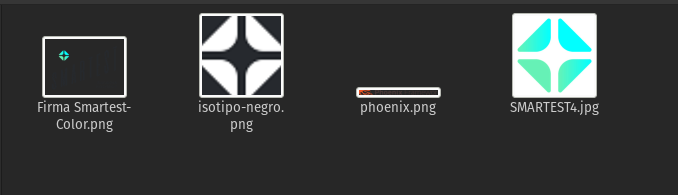
\includegraphics[width=0.7\textwidth]{capitulo2/imagenes.png}
\caption{Logos de SMARTEST en el directorio \textbf{jitro\_ui /assets /static /images}}
\label{cap2:002}
\end{figure}

Ahora editaremos el archivo jitro\_ui /lib /jitro\_ui\_web /templates /layout /root.html.leex

\begin{lstlisting}[language=html]
<!DOCTYPE html>
<html lang="en">
  <head>
    <meta charset="utf-8"/>
    <meta http-equiv="X-UA-Compatible" content="IE=edge"/>
    <meta name="viewport" content="width=device-width, initial-scale=1.0"/>
    <%= csrf_meta_tag() %>
    <%= live_title_tag assigns[:page_title] || "Jitro", suffix: "Sistema de acceso" %>
    <link phx-track-static rel="stylesheet" href="<%= Routes.static_path(@conn, "/css/app.css") %>"/>
    <script defer phx-track-static type="text/javascript" src="<%= Routes.static_path(@conn, "/js/app.js") %>"></script>
  </head>
  <body>
    <header>
      <section class="container">
        <nav role="navigation">
          <ul>
            <li><a href="http://www.smartest.mx/">Pagina de inicio</a></li>
            <%= if function_exported?(Routes, :live_dashboard_path, 2) do %>
              <li><%= link "LiveDashboard", to: Routes.live_dashboard_path(@conn, :home) %></li>
            <% end %>
          </ul>
        </nav>
        <a href="https://www.smartest.mx/" class="phx-logo">
          <img src="<%= Routes.static_path(@conn, "/images/SMARTEST3.jpg") %>" alt="Logo SMARTEST"/>
        </a>
      </section>
    </header>
    <%= @inner_content %>
  </body>
</html>
\end{lstlisting}

El resultado se muestra en la figura \ref{cap2:003}.
\begin{figure}[htb]
\centering
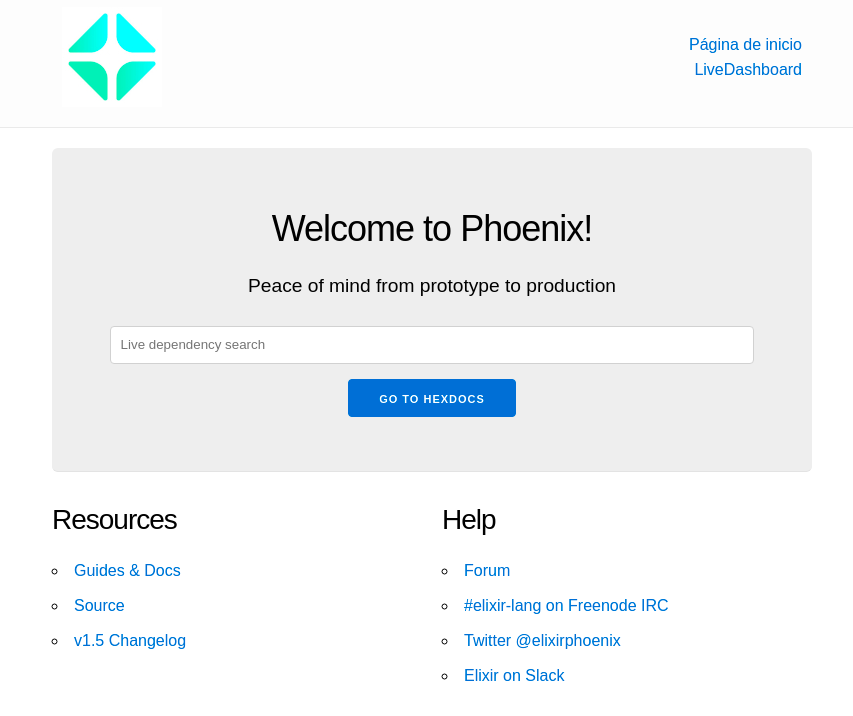
\includegraphics[width=0.7\textwidth]{capitulo2/primeraPantalla.png}
\caption{Pantalla de accesos después de la modificación}
\label{cap2:003}
\end{figure}

Ahora eliminamos la bienvenida de Phoenix para colocar nuestros letreros, para ello editamos el archivo jitro\_ui /lib /jitro\_ui\_web /live /page\_live.html.leex, como se muestra:

\begin{lstlisting}[language=html]
<section class="phx-hero">
  <h1><%= gettext "Bienvenido a %{name}!", name: "Jitro" %></h1>
  <p>El sistema de control de accesos de SMARTEST</p>


</section>

<section class="row">
  <article class="column">
    <h2>Recursos</h2>

  </article>
  <article class="column">
    <h2>Ayuda</h2>

  </article>
</section>
\end{lstlisting}

Quedando como se muestra en la figura \ref{cap2:004}

\begin{figure}[htb]
\centering
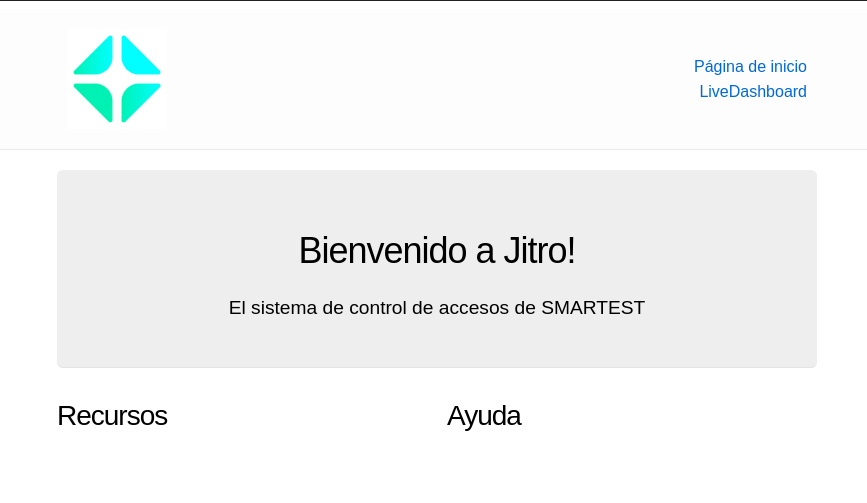
\includegraphics[width=0.7\textwidth]{capitulo2/bienvenida.png}
\caption{Pantalla de accesos después de la modificación de bienvenida}
\label{cap2:004}
\end{figure}

\section{Lectura a través de HID}

Los dispositivos HID (\textbf{\emph{Human Interface Devices}}) pueden ser de dos tipos principales:

\begin{itemize}
\item Los HIDRAW.- El controlador hidraw proporciona una interfaz sin formato para dispositivos de interfaz humana USB y Bluetooth. Se diferencia de hiddev en que los informes enviados y recibidos no son analizados por el analizador HID, sino que se envían y reciben del dispositivo sin modificar.
\item Los HIDDEV.- 
\end{itemize}

\subsection{hidraw}

Hidraw debe utilizarse si la aplicación del espacio de usuario sabe exactamente cómo
comunicarse con el dispositivo de hardware y puede construir los informes HID manualmente. Este suele ser el caso cuando se crean controladores de espacio de usuario para dispositivos HID personalizados.

Hidraw también es útil para comunicarse con dispositivos HID no conformes que envían y reciben datos de una manera que no concuerda con sus descriptores de informes. Debido a que hiddev analiza los informes que se envían y reciben a través de él, comparándolos con el descriptor de informes del dispositivo, dicha comunicación con estos dispositivos no conformes es imposible utilizando hiddev. Hidraw es la única alternativa, además de escribir un controlador de kernel personalizado, para estos dispositivos no compatibles.

Un beneficio de hidraw es que su uso por parte de las aplicaciones del espacio de usuario es independiente del tipo de hardware subyacente. Actualmente, Hidraw está implementado para USB y Bluetooth. En el futuro, a medida que se desarrollen nuevos tipos de bus de hardware que utilicen la especificación HID, hidraw se ampliará para agregar soporte para estos nuevos tipos de bus.

Hidraw usa un número mayor dinámico, lo que significa que se debe confiar en udev para crear nodos de dispositivo hidraw. Udev normalmente creará los nodos del dispositivo directamente debajo de / dev (por ejemplo: / dev / hidraw0). Como esta ubicación depende de la distribución y de las reglas de udev, las aplicaciones deben usar libudev para ubicar los dispositivos hidraw conectados al sistema.

\subsection{hiddev}

Además de los dispositivos HID de tipo de entrada normal, USB también utiliza los protocolos de dispositivo de interfaz humana para cosas que no son realmente interfaces humanas, pero que tienen necesidades de comunicación similares. Los dos grandes ejemplos de esto son los dispositivos de alimentación (especialmente las fuentes de alimentación ininterrumpidas) y el control del monitor en monitores de gama alta.

Para admitir estos requisitos dispares, el sistema USB de Linux proporciona eventos HID a dos interfaces separadas:

\begin{itemize}
\item el subsistema de entrada, que convierte los eventos HID en interfaces de dispositivos de entrada normales (como teclado, mouse y joystick) y una interfaz de eventos normalizada; consulte Documentation / input / input.rst
\item la interfaz hiddev, que proporciona eventos HID bastante crudos
\end{itemize}

El flujo de datos para un evento HID producido por un dispositivo es similar al que se muestra en la figura \ref{cap2:005}

\begin{figure}[htb]
\centering
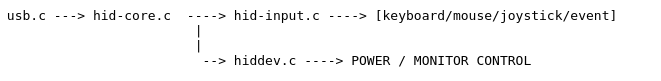
\includegraphics[width=0.8\textwidth]{capitulo2/hid_seq.png}
\caption{Flujo de datos para un evento HID}
\label{cap2:005}
\end{figure}

Además, otros subsistemas (además de USB) pueden potencialmente alimentar eventos en el subsistema de entrada, pero estos no tienen ningún efecto en la interfaz del dispositivo oculto.

La interfaz hiddev es una interfaz de caracteres que utiliza el USB mayor normal, con los números menores comenzando en 96 y terminando en 111. Por lo tanto, necesita los siguientes comandos:

\begin{lstlisting}[language=bash]
mknod /dev/usb/hiddev0 c 180 96
mknod /dev/usb/hiddev1 c 180 97
mknod /dev/usb/hiddev2 c 180 98
mknod /dev/usb/hiddev3 c 180 99
mknod /dev/usb/hiddev4 c 180 100
mknod /dev/usb/hiddev5 c 180 101
mknod /dev/usb/hiddev6 c 180 102
mknod /dev/usb/hiddev7 c 180 103
mknod /dev/usb/hiddev8 c 180 104
mknod /dev/usb/hiddev9 c 180 105
mknod /dev/usb/hiddev10 c 180 106
mknod /dev/usb/hiddev11 c 180 107
mknod /dev/usb/hiddev12 c 180 108
mknod /dev/usb/hiddev13 c 180 109
mknod /dev/usb/hiddev14 c 180 110
mknod /dev/usb/hiddev15 c 180 111
\end{lstlisting}

\subsection{Puertos HID del lector}

Cuando conectamos el lector de QR, RFID y NFC en un puerto USB, podemos detectalo usando el comando que se muestra en la figura \ref{cap2:006}.

\begin{figure}[htb]
\centering
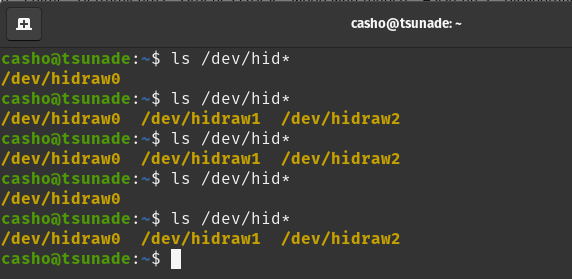
\includegraphics[width=0.8\textwidth]{capitulo2/listaHID.png}
\caption{Lista de dispositivos HID cuando conectas un lector}
\label{cap2:006}
\end{figure}

En la figura \ref{cap2:006} se muestra el resultado del comando \textbf{ls /dev/hid*} cuando se conecta y desconecta un lector. Debe revisarse en cual puerto de los dos que activa el lector, envia los datos de sus tres métodos de lectura: QR, RFID y NFC.

La captura de las lecturas a través del puerto \textbf{/dev/hidrawX} se realizan utilizando dos Genservers y un programa: 

\begin{itemize}
\item Programa \textbf{lector.ex} .- El programa tiene dos mapas y dos rutinas. Los mapas convierten el número hexadecimal que lee el puerto HID y lo convierte en un caracter utf-8, el mapa \textbf{@hid} los convierte el minúsculas y el \textbf{@hid2} los convierte en mayúsculas. La función \textbf{decode\_hid} lee la secuencia hexadecimal de un caracter, la cual viene formada por muchos ceros y algún codigo hexadecimal de la tecla enter (un solo número diferente) o un número hexadecimal diferente que representa una caracter o bien dos número hexadecimal que representan un letra mayúscula (ya que uno de esos dos números es el código de la tecla shift). La función \textbf{generar} primero filtra los ceros del lector, posteriormente convierte los codigos hexadecimal leídos en caracteres utf-8 y por último filtra aquellos caracteres vacios.
\item Genserver lector\_hid1.ex .- Este genserver abre el puerto para leer los hexadecimales de entrada del lector y va creando en su estado la lista de caracteres utf-8 que corresponden a cada lista de hexadecimales leídos. Además concatena la lista de caracteres para formar la cadena de lectura. Envia al genserver cadena\_actual la cadena leida y si esta corresponde a un lector de entrada o de salida, basandose en el numero de puerto HID que hizo la lectura.
\item Genserver \textbf{cadena\_actual.ex} .- Este genserver mantiene en su estado la última cadena leída y que lector la realizó: si el de entrada o salida.
\end{itemize}

A continuación se muestra el código del programa \textbf{lector.ex}

\subsubsection{Código del programa lector.ex}

\begin{lstlisting}[language=erlang]
defmodule JitroUi.Lector do
  # ***************** Teclas Especiales **************
  #define KEY_MOD_RSHIFT 0x20
  #define KEY_MOD_LSHIFT 0x02
  @shift_derecha    0x20
  @shift_izquierda  0x02
  @enter            0x28

  @hid %{ 0x04 => 'a',
          0x05 => 'b',
          0x06 => 'c',
          0x07 => 'd',
          0x08 => 'e',
          0x09 => 'f',
          0x0A => 'g',
          0x0B => 'h',
          0x0C => 'i',
          0x0D => 'j',
          0x0E => 'k',
          0x0F => 'l',
          0x10 => 'm',
          0x11 => 'n',
          0x12 => 'o',
          0x13 => 'p',
          0x14 => 'q',
          0x15 => 'r',
          0x16 => 's',
          0x17 => 't',
          0x18 => 'u',
          0x19 => 'v',
          0x1A => 'w',
          0x1B => 'x',
          0x1C => 'y',
          0x1D => 'z',
          0x1E => '1',
          0x1F => '2',
          0x20 => '3',
          0x21 => '4',
          0x22 => '5',
          0x23 => '6',
          0x24 => '7',
          0x25 => '8',
          0x26 => '9',
          0x27 => '0',
          0x2C => ' ',
          0x2D => '-',
          0x2E => '=',
          0x2F => '[',
          0x30 => ']',
          0x31 => '\\',
          0x33 => ';' ,
          0x34 => '\'',
          0x35 => '`',
          0x36 => ',',
          0x37 => '.',
          0x38 => '/' ,
          0x28 => '' }
  @hid2 %{ 0x04 => 'A',
          0x05 => 'B',
          0x06 => 'C',
          0x07 => 'D',
          0x08 => 'E',
          0x09 => 'F',
          0x0A => 'G',
          0x0B => 'H',
          0x0C => 'I',
          0x0D => 'J',
          0x0E => 'K',
          0x0F => 'L',
          0x10 => 'M',
          0x11 => 'N',
          0x12 => 'O',
          0x13 => 'P',
          0x14 => 'Q',
          0x15 => 'R',
          0x16 => 'S',
          0x17 => 'T',
          0x18 => 'U',
          0x19 => 'V',
          0x1A => 'W',
          0x1B => 'X',
          0x1C => 'Y',
          0x1D => 'Z',
          0x1E => '!',
          0x1F => '@',
          0x20 => '#',
          0x21 => '$',
          0x22 => '%',
          0x23 => '^',
          0x24 => '&',
          0x25 => '*',
          0x26 => '(',
          0x27 => ')',
          0x2C => ' ',
          0x2D => '_',
          0x2E => '+',
          0x2F => '{',
          0x30 => '}',
          0x31 => '|',
          0x33 => ':' ,
          0x34 => '"',
          0x35 => '~',
          0x36 => '<',
          0x37 => '>',
          0x38 => '?' ,
          0x28 => '' }
  def generar(mensaje) do
    mensaje
      |> Enum.filter(fn y -> y > 0 end )
      |> decode_hid
      |> Enum.filter(fn y -> y != [] end )
  end

  @spec decode_hid(nonempty_maybe_improper_list, any) :: [[1..255]]
  def decode_hid(lista, shift \\ false) do
    if (lista != []) do
            valores= Enum.reduce(lista, 0, fn x, acc -> x + acc end)
            [h|t] = lista
            if (h == @enter ) do
              ''
            else
              {cadena, shift2} =  if (h == @shift_derecha || h == @shift_izquierda) && (valores > 0x20) do
                                    {'', true}
                                  else
                                    if shift == true do
                                      case Map.fetch(@hid2, h) do
                                        {:ok, dato} -> {dato, false}
                                        _  ->  {'', false}
                                      end
                                    else
                                      case Map.fetch(@hid, h) do
                                        {:ok, dato} -> {dato, false}
                                                _  ->  {'', false}
                                      end
                                    end
                                  end
              [cadena | decode_hid(t, shift2)]
            end
    else
      ''
    end
  end
end

\end{lstlisting}

Ahora el código del genserver \textbf{lector\_hid1.ex}

\subsubsection{Código del genserver lector\_hid1.ex}

\begin{lstlisting}[language=erlang]
defmodule JitroUi.LectorHid1 do
  use GenServer
  alias JitroUi.Lector
  alias JitroUi.CadenaActual

  @nombre :lectorHID1_server
  @valor_inicial []

  def start_link(_opts) do
    GenServer.start_link(__MODULE__, @valor_inicial, name: @nombre)
  end
  def init(lista_inicial) do
    _pid = Port.open('/dev/hidraw1', [:stream, :eof])
    {:ok, lista_inicial}
  end
  def actualizar() do
    GenServer.call @nombre, :actualizar
  end

  def actual() do
    GenServer.call @nombre, :actual
  end
  def handle_call(:actual, _from, ultima_lectura) do
    {:reply, ultima_lectura, ultima_lectura}
  end
  def handle_call(:actualizar, _from, ultima_lectura) do
    {:reply, ultima_lectura, ultima_lectura}
  end
  def handle_info(mensaje, estado) do
    {_puerto, {:data, caracter}} = mensaje
    nuevo_caracter =  caracter
      |> Enum.filter(fn y -> y > 0 end )
    nuevo_estado =  if nuevo_caracter != [] do
                      if Enum.any?(caracter, fn y -> y == 40 end) do
                        IO.puts "\n Cadena Salida: "
                        IO.puts (inspect estado)
                        CadenaActual.actualizar({estado,"entrada" })
                        []
                      else
                        #IO.puts Lector.generar(caracter)
                        generado=Lector.generar(caracter)
                        #IO.puts "#{estado}+#{generado}"
                        #IO.puts (inspect caracter)
                        [estado | generado]
                      end
                    else
                      estado
                    end
    {:noreply,  List.flatten( nuevo_estado)}
  end
end
\end{lstlisting}

Por último el código de \textbf{cadena\_actual.ex}

\subsubsection{Código del genserver \textbf{cadena\_actual.ex}}

\begin{lstlisting}[language=erlang]
defmodule JitroUi.CadenaActual do
  use GenServer

  @nombre :cadenaActual_server
  @valor_inicial %{:lectura =>"Aun no lee ", :direccion =>"Sin direccion "}

  def start_link(_opts) do
    GenServer.start_link(__MODULE__, @valor_inicial, name: @nombre)
  end
  def init(lista_inicial) do
    {:ok, lista_inicial}
  end
  def actual() do
    GenServer.call @nombre, :actual
  end
  def actualizar(lectura) do
    GenServer.call @nombre, {:actualizar, lectura}
  end
  def handle_call(:actual, _from, respuesta) do
    {:reply, respuesta, respuesta}
  end
  def handle_call({:actualizar,{cadena, direccion}}, _from, _lector) do
    estado_actual=%{:lectura => cadena, :direccion => direccion}
    {:reply, estado_actual, estado_actual}
  end
end
\end{lstlisting}

\section{Captura de datos del lector}

Para la captura de los datos del lector es necesario editar el archivo \textbf{jitro\_ui /lib /jitro\_ui\_web /live /page\_live.ex} y borrar las rutinas no utilizadas, quedando solo la rutina \textbf{mount} la cual editamos y permitimos la transferencia de un mapa que llamaremos ultima\_lectura que tendrá la siguiente estructura:

\begin{lstlisting}[language=erlang]
%{
	:lectura => cadena,
	:direccion => direccion
}
\end{lstlisting}

El archivo el archivo \textbf{jitro\_ui/lib/jitro\_ui\_web/live/page\_live.ex} queda de la siguiente fomra:

\begin{lstlisting}[language=erlang]
defmodule JitroUiWeb.PageLive do
  use JitroUiWeb, :live_view

  @impl true
  def mount(_params, _session, socket) do
    if connected?(socket), do: Process.send_after(self(), :actualizar, 100)

    {:ok, assign(socket, resultado: %{ :lectura => "Aun no lee", :direccion => "Sin direccion"})}
  end

  def handle_info(:actualizar, socket) do
    Process.send_after(self(), :actualizar, 100)
    lectura = JitroUi.CadenaActual.actual
    {:noreply, assign(socket, :resultado, lectura)}
  end

end
\end{lstlisting}

Asi mismo, es necesario modificar el archivo \textbf{jitro\_ui /lib /jitro\_ui\_web /live /page\_live.html.leex}

\begin{lstlisting}[language=erlang]
<section class="phx-hero">
  <h1><%= gettext "Bienvenido a %{name}!", name: "Jitro" %></h1>
  <p>El sistema de control de accesos de SMARTEST</p>


</section>

<section class="row">
  <article class="column">
    <h2>Lectura</h2>
    <%= @resultado.lectura %> 
  </article>
  <article class="column">
    <h2>Direccion</h2>
    <%= @resultado.direccion %>
  </article>
</section>
\end{lstlisting}

Para que los \textbf{genservers} de lectura esten activos es necesario darlos de alta en el archivo \textbf{jitro\_ui /lib /jitro\_ui /aplication.ex} quedando de la siguiente forma:

\begin{lstlisting}[language=erlang]
...
  def start(_type, _args) do
    children = [
      JitroUi.CadenaActual,
      JitroUi.LectorHid1,

      # Start the Telemetry supervisor
      JitroUiWeb.Telemetry,
      # Start the PubSub system
      {Phoenix.PubSub, name: JitroUi.PubSub},
      # Start the Endpoint (http/https)
      JitroUiWeb.Endpoint
      # Start a worker by calling: JitroUi.Worker.start_link(arg)
      # {JitroUi.Worker, arg}
    ]
...
\end{lstlisting}

